%%%%%%%%%%%%%%%%%%%%%%%%%%%%%%%%%%%%%%%%%%%%%%%%%%
%%%%%%%%%%
% Document preamble

% Document type
\documentclass[11pt, twoside]{article}
\usepackage[utf8]{inputenc}

% Document layout dimensions
%\usepackage[letterpaper, portrait, margin=1in]{geometry}
\usepackage{geometry}
\geometry{letterpaper, portrait, margin=2cm}

% Document header and footer
% https://www.sharelatex.com/learn/Headers_and_footers
% https://www.ctan.org/pkg/fancyhdr?lang=en
% Commands \pagestyle and \pagenumbering are native to latex.
% Package fancyhdr provides additional ease and control.
\usepackage{fancyhdr}
\setlength{\headheight}{14pt}
% Include headers and footers in both fancy and plain page styles
% so that the first pages of chapters will have headers and footers.
% For any page of the document set the page style using commands.
%\thispagestyle{empty}
%\thispagestyle{plain}
%\thispagestyle{headings}
%\thispagestyle{myheadings}
%\thispagestyle{fancy}

%\pagestyle{fancy}
%\lhead{}
%\chead{}
%\rhead{}
%\lfoot{}
%\cfoot{}
%\rfoot{\thepage}
%\fancyhf{}
%\fancyhead{}
%\fancyhead[L]{Profondeur}
%\fancyhead[R]{Visual Exploration and Analysis of Metabolic Networks}
%\fancyfoot{}
%\fancyfoot[L]{Chapter \thechapter}
%\fancyfoot[C]{T Cameron Waller}
%\fancyfoot[R]{Page \thepage}
\renewcommand{\headrulewidth}{0.5pt}
\renewcommand{\footrulewidth}{0.5pt}

% Document font
%\renewcommand{\familydefault}{\rmdefault}
\renewcommand{\familydefault}{\sfdefault}
%\rmfamily
%\sffamily
%\ttfamily

\setcounter{secnumdepth}{0}
\usepackage{indentfirst}

% figures
% https://www.sharelatex.com/learn/Inserting_Images


\usepackage{graphicx}
\graphicspath{ {figures/} }


%\begin{figure}[t]
%\centering
%\includegraphics{file name without suffix}
%\includegraphics[scale=1.5]{file name without suffix}
% scale image dimensions by document property
%\includegraphics[width=\textwidth]{file name without suffix}
%\includegraphics[width=8cm]{Plot}
%\caption{}
%\label{fig:figure_reference}
%\end{figure}
%\ref{fig:figure_reference}

% table
\usepackage{array}
\usepackage{multirow}
\setlength{\tabcolsep}{0.1cm}
\renewcommand{\arraystretch}{1.5}
%\begin{table}[t]
%\centering
%\begin{tabular}{ |c|c|c| }
%\hline
%cell1 & cell2 & cell3 \\
%\hline
%cell4 & cell5 & cell6 \\
%\hline
%cell7 & cell8 & cell9 \\
%\hline
%\end{tabular}
%\caption{}
%\label{table:concepts}
%\end{table}
%\ref{table:concepts}

% Support reference citations
\usepackage[backend=biber, sorting=none]{biblatex}
\addbibresource{reference.bib}
%\bibliographystyle{unsrt}

% Project title, author, and date
\title{design_proposal}
\author{Thomas Cameron Waller}
\date{\today}

%%%%%%%%%%
% Format notes

% block comments
%\usepackage{comment}
%\begin{comment}
%\end{comment}

%\hyphenation{unusual-word}
%unusual\word

% text justification
%\begin{center} %\centering
%\end{center}
%\begin{flushleft} %\raggedright
%\end{flushleft}
%\begin{flushright} %\raggedleft
%\end{flushright}

% paragraph indentation
%\setlength{\parindent}{10ex}
%\indent
%\noindent

% paragraph break
%\par

% line break
% \\
% \\*
% \newline
%\hfill \break
%\linebreak[number0-4] % priority 0-4 for optimal formatting

% page break
%\newpage
%\clearpage

% horizontal blank space
%\hspace{1cm} % other units work, too
%\hfill
%\hrulefill
%\dotfill

% vertical blank space
%\vspace{5mm}
%\vfill
%\smallskip
%\medskip
%\bigskip

% document sections
%\chapter{Name}
%\section{Name}
%\paragraph{Name}

% font
%\textbf{text}
%\textit{text}

% citation
%\supercite{reference}
%\printbibliography

%%%%%%%%%%
% references
% https://www.sharelatex.com/learn/
% https://www.sharelatex.com/learn/Font_sizes,_families,_and_styles
% https://www.sharelatex.com/learn/Font_typefaces
% https://www.sharelatex.com/learn/Lists
% https://www.sharelatex.com/learn/Bibliography_management_in_LaTeX
% https://www.sharelatex.com/learn/Tables
% https://www.sharelatex.com/learn/Positioning_images_and_tables
% http://tex.stackexchange.com/questions/39017/how-to-influence-the-position-of-float-environments-like-figure-and-table-in-lat
% https://www.latex-project.org/publications/#publications-in-2014

%%%%%%%%%%%%%%%%%%%%%%%%%%%%%%%%%%%%%%%%%%%%%%%%%%

%%%%%%%%%%
% document body
\begin{document}

%%%%%%%%%%
% I need to be careful of my terminology.
% I need to consider when and where to use "system" or "network".

%%%%%%%%%%
% Title
%%%%%%%%%%%%%%%%%%%%%%%%%%%%%%%%%%%%%%%%%%%%%%%%%%

%%%%%%%%%%
% Create title page for document.

\begin{titlepage}
\begin{center}

% Title
\vspace*{2cm}
\Huge
\textbf{Profondeur}

% Subtitle
\vspace{0.5cm}
\LARGE
Visual Exploration and Analysis of Metabolic Networks

% Author
\vspace{1.5cm}
\LARGE
\textbf{T Cameron Waller}

% Date
%\today
\vspace{1.5cm}
\Large
\textbf{2 December 2016}


% Context
\vfill
\Large
Course Project\\
University of Utah\\
Data Visualization\\
Alexander Lex\\
Fall 2016

\end{center}
\end{titlepage}

%%%%%%%%%%
% summary
%%%%%%%%%%%%%%%%%%%%%%%%%%%%%%%%%%%%%%%%%%%%%%%%%%
%%%%%%%%%%

% summary

\section{Summary}

Metabolism is a vast and complex system with many types of relations between many types of biological entities.
With extensive connections throughout, it functions as a cooperative network.
To scientists, engineers, and clinicians who study metabolism, this complexity and continuity present a great challenge.
Investigators need to consider the holistic context of the network in order both to design experiments reliably and interpret experimental results accurately.
Current technologies for exploring metabolism primarily divide the network into distinct pathways and show these in static maps.
These tools fail to represent the continuity of the metabolic network as a whole.
They also fail to support exploration according to case-specific interest.
The goal of this project is to develop computational methods and a tool to enable users to explore the metabolic network.
In contrast to current technologies, this tool will support queries against the entire network to define custom selections.
This tool will represent these selections dynamically, offering alternative views to illustrate properties and attributes clearly.

%%%%%%%%%%
% introduction
%%%%%%%%%%%%%%%%%%%%%%%%%%%%%%%%%%%%%%%%%%%%%%%%%%
%%%%%%%%%%
% introduction

\section{Introduction}

% describe the scope/goal of the project

%metabolism
% metabolism is fundamental part of biological system.
% metabolism is a network.
% metabolism functions a a cooperative and continuous whole.
% metabolic defects drive many human diseases.

\textbf{Metabolism} is an integral part of the biological systems of cells, tissues, and organisms.
\textbf{Catabolic processes} degrade food to liberate energy and materials.
\textbf{Anabolic processes} utilize these materials and harness this energy to synthesize all cellular components.
In this way, \textbf{metabolism sustains life and all of its diverse processes}.
It is little wonder that metabolic defects contribute to the pathology of many human diseases, including obesity, diabetes, cardiovascular disease, and cancer \supercite{van_der_klaauw_hunger_2015, haslam_obesity_2005}.

\textbf{Metabolism is a cooperative and continuous system}.
In the cell, tens of thousands of different types of \textbf{genes, transcripts, proteins, and metabolites} exist in various amounts in separate compartments.
These \textbf{compartments partition the cell into environments with specific purposes}.
Genes and transcripts encode proteins, and proteins have many functions.
\textbf{Proteins transport metabolites between compartments and catalyze chemical reactions between metabolites}, performing these tasks with exceptional precision.
They control and regulate the rates and compartments of transports or reactions as well as which metabolites participate.
Metabolites, in turn, are the fuel and building blocks of cells.
All of these diverse functions influence each other such that \textbf{local modifications can impart pervasive effects throughout the system}.

% study of metabolism
% users

The study of metabolism is changing.
Traditionally this study involved experts who conducted \textbf{reductionist experiments} to characterize the functions of individual genes, transcripts, proteins, and metabolites.
Over many years, many of these experiments have contributed sufficient knowledge to consider the \textbf{greater perspective of pathways, processes and entire systems} \supercite{wang_systems_2015}.
Modern technologies, especially the \textbf{omics technologies (genomics, transcriptomics, proteomics, and metabolomics)} measure these systems at nearly comprehensive scales and provide rich information \supercite{zhang_forward_2015}.
Also, there is an increase in \textbf{interest and accessibility} such that the study of metabolism is becoming more \textbf{interdisciplinary}.
Scientists and engineers from diverse backgrounds consider metabolic mechanisms and phenotypes, and metabolic profiling in the clinic is an important goal towards \textbf{precision medicine} \supercite{beebe_sharpening_2016, benson_clinical_2016, tebani_omics-based_2016, collins_new_2015, wang_systems_2015, zhang_forward_2015, topol_individualized_2014}.

% challenges

These changes present challenges and opportunities.
The modern study of metabolism needs an \textbf{holistic perspective}, such as that of the discipline of \textbf{systems biology}.
Only this perspective sufficiently considers the \textbf{real context} in order to \textbf{design experiments reliably and interpret experimental results accurately}.
However, the vastness and complexity of metabolism exceed even the ability of experts to understand in its entirety.
Novice and expert investigators alike need tools to study the metabolic system.
The goal of this project is to develop \textbf{computational methods and a tool to support the study of metabolism}.


%%%%%%%%%%
% requirements
%%%%%%%%%%%%%%%%%%%%%%%%%%%%%%%%%%%%%%%%%%%%%%%%%%
%%%%%%%%%%

% requirements
% describe users (including their domains) here in more detail
% user needs
% tasks

\section{Requirements}

% figures

% tables

%%%%%%%%%%%%%%%%%%%%%%%%%%%%%%%%%%%%%%%%%%%%%%%%%%
%%%%%%%%%%
% table concept

% table
\begin{table}[htbp]
\small
\centering
\begin{tabular}{ |m{1.9cm}|m{11cm}|m{1cm}|m{1.3cm}|m{1cm}| }
% column header
\hline
\textbf{Category}
& \textbf{Concept}
& \textbf{Expert}
& \textbf{Inter\-mediate}
& \textbf{Novice}
\\
% encoding
\hline
\multirow{3}{1.5cm}{\textbf{Encoding}}
& \textbf{Genes} encode \textbf{transcripts} via \textbf{transcription}.
& \textbf{X}
& \textbf{X}
& \textbf{X}
\\
\cline{2-5}
& \textbf{Transcripts} encode \textbf{proteins} via \textbf{translation}.
& \textbf{X}
& \textbf{X}
& \textbf{X}
\\
\cline{2-5}
& \textbf{Proteins} mediate both \textbf{transcription} and \textbf{translation}.
& \textbf{X}
& \textbf{X}
&
\\
% expression
\hline
\multirow{2}{1.5cm}{\textbf{Expression}}
& \textbf{Proteins} regulate the extent of both \textbf{transcription} and \textbf{translation} via interaction with \textbf{genes}, \textbf{transcripts}, and other \textbf{proteins}.
& \textbf{X}
& \textbf{X}
&
\\
\cline{2-5}
& \textbf{Metabolites} regulate the extent of both \textbf{transcription} and \textbf{translation} via interaction with \textbf{proteins}.
& \textbf{X}
&
&
\\
% reaction
\hline
\multirow{8}{1.5cm}{\textbf{Reaction}}
& \textbf{Reactions} involve a chemical change between \textbf{metabolites}.
& \textbf{X}
& \textbf{X}
& \textbf{X}
\\
\cline{2-5}
& \textbf{Reactants} are \textbf{metabolites} that participate in the start of a \textbf{reaction}.
& \textbf{X}
& \textbf{X}
& \textbf{X}
\\
\cline{2-5}
& \textbf{Products} are \textbf{metabolites} that participate in the end of a \textbf{reaction}.
& \textbf{X}
& \textbf{X}
& \textbf{X}
\\
\cline{2-5}
& Some \textbf{metabolites} participate in more \textbf{reactions} than others.
& \textbf{X}
& \textbf{X}
&
\\
\cline{2-5}
& \textbf{Reactions} have different \textbf{rates}.
& \textbf{X}
&
&
\\
\cline{2-5}
& \textbf{Reactions} have different \textbf{directions} and likelihoods/probabilities of \textbf{reversibility}.
& \textbf{X}
&
&
\\
\cline{2-5}
& \textbf{Pathways} are sets of multiple \textbf{reactions} that carry out major processes.
& \textbf{X}
& \textbf{X}
&
\\
\cline{2-5}
& \textbf{Reactions} between \textbf{metabolites} make a cooperative and continuous network.
& \textbf{X}
&
&
\\
% catalysis
\hline
\multirow{1}{1.5cm}{\textbf{Catalysis}}
& \textbf{Proteins} catalyze \textbf{reactions} between \textbf{metabolites}.
& \textbf{X}
& \textbf{X}
&
\\
% transport
\hline
\multirow{2}{1.5cm}{\textbf{Transport}}
& \textbf{Membranes} partition the eukaryotic \textbf{cell} into separate \textbf{compartments}.
& \textbf{X}
& \textbf{X}
& \textbf{X}
\\
\cline{2-5}
& \textbf{Proteins} mediate \textbf{transport} of \textbf{metabolites} between \textbf{compartments}.
& \textbf{X}
& \textbf{X}
&
\\
% regulation
\hline
\multirow{4}{1.5cm}{\textbf{Regulation}}
& Multiple copies of the same \textbf{transcript}, \textbf{protein}, or \textbf{metabolite} are present in the cell in dynamic \textbf{pools} of variable amounts.
& \textbf{X}
& \textbf{X}
&
\\
\cline{2-5}
& \textbf{Metabolites} regulate the extent of \textbf{catalysis} and \textbf{transport} via interaction with \textbf{proteins}.
& \textbf{X}
&
&
\\
\cline{2-5}
& \textbf{Proteins} regulate the extent of \textbf{catalysis} and \textbf{transport} via interaction with other \textbf{proteins}.
& \textbf{X}
& \textbf{X}
&
\\
\cline{2-5}
& Changes to a single \textbf{metabolite} or \textbf{reaction} can influence others even great distances away in the network.
& \textbf{X}
&
&
\\
% technology
\hline
\multirow{3}{1.5cm}{\textbf{Technology}}
& \textbf{'Omics} technologies identify modifications to \textbf{genes}, \textbf{transcripts}, or \textbf{proteins}.
& \textbf{X}
& \textbf{X}
&
\\
\cline{2-5}
& \textbf{'Omics} technologies measure the abundances of \textbf{transcripts}, \textbf{proteins}, or \textbf{metabolites} in a sample and thereby suggest the pool amount in a cell.
& \textbf{X}
& \textbf{X}
&
\\
\cline{2-5}
& To compare relative abundances from multiple samples, it is necessary to consider any differences in \textbf{conditions} or \textbf{parameters}.
& \textbf{X}
&
&
\\
% science
\hline
\multirow{1}{1.5cm}{\textbf{Science}}
& \textbf{Experiments} require specific controls to study specific variables.
& \textbf{X}
& \textbf{X}
&
\\
\hline
\end{tabular}
\caption{Fundamental biological, technological, and scientific concepts relevant to the study of metabolism.}
\label{table:concept}
\end{table}



% users
% diverse backgrounds
% diverse levels of interest in metabolism
% common need to design experiments and interpret results
% diverse computational knowledge (keep it simple)

The target \textbf{users} of this project's tool have diverse expertise and interest in the study of metabolism.
They are scientists, engineers, or clinicians in the domains of \textbf{biology, biotechnology, pharmacology, or medicine}.
\textbf{Experts} are scientists or engineers who understand both general biology and specific metabolism thoroughly.
Their interest is either to discover new processes within this system or to modify it for some therapeutic or synthetic benefit.
They understand relevant methods and technologies and know how to use them properly in experimentation.
\textbf{Intermediates} are scientists or engineers who understand general biology but are less familiar with specific metabolism.
Their interest is to consider some aspects of metabolism that relate to another subject.
They also understand relevant methods and technologies and know how to use them properly in experimentation.
\textbf{Novices} are scientists, engineers, or clinicians who understand only basic, general biology.
Their interest is also to consider some aspects of metabolism that relate to another subject.
Their interest may even be to profile the metabolism of a patient in order to diagnose a disease or prescribe an appropriate therapy.
They do not understand relevant technologies or how to use them properly in experimentation.
\textbf{Table \ref{table:concept}} describes how these categories of users understand fundamental concepts in the study of metabolism.

% user needs

For all users, the study of metabolism has some general requirements.
Broadly, users' goals are \textbf{1) to design experiments reliably} and \textbf{2) to interpret experimental results accurately}.
Both of these goals require appropriate consideration for the context of the subject in study.
Since \textbf{metabolism is a continuous system that functions cooperatively}, the real context is the entire system, but its vastness and complexity are inaccessible.
To handle vastness, \textbf{users need information in detail for narrow selections without neglecting the broad context}.
To handle complexity, \textbf{users need to explore different types of information in different ways}.
In both cases, they need \textbf{flexibility to match their interest}.

%%%%%%%%%%
%%%%%%%%%%
%%%%%%%%%%

% selection requirements

\subsection{Selection Requirements}
Metabolism is a vast system.
The user needs to select portions of the metabolic system that are sufficiently simple to conceptualize in detail yet sufficiently inclusive to give accurate context.
These selections need to match the user's interest appropriately.

\begin{enumerate}

\item \textbf{Select portions of the metabolic system by how they relate to a set of entities of interest.}
\\
The user has interest in single or multiple entities (genes, transcripts, proteins, or metabolites) and needs information about these entities and also about other entities that relate to them.
This selection must be appropriate for the user's custom, case-specific interest.
It must be independent of typical pathways or other categories since interest often traverses or transcends these pathways.

\item \textbf{Select portions of the metabolic system that either have or do not have some specific property or attribute.}
\\
Entities have many \textbf{biological properties}.
They also can have \textbf{attributes from experimental measurements} such as fold change in abundance or p-value.
The user needs to identify entities that have or do not have some specific properties or attributes.

\item \textbf{Select portions of the metabolic system both by their relations and by their properties or attributes.}
\\
Combining selection criteria can be much more specific.
In particular, the user might have a list of entities with properties and attributes.
The user might only have interest in entities with certain properties and attributes from this list, for which they need information and context.

\item \textbf{Refine selection by inclusion or exclusion of individual entities.}
\\
The user needs to define very specific selections.
Direct selection of individual entities might be necessary if more general selections are too ambiguous.

\end{enumerate}

%%%%%%%%%%
%%%%%%%%%%
%%%%%%%%%%

% exploration tasks

\subsection{Exploration Requirements}
Metabolism is a complex system in that many types of entities and relations have many types of properties.
There is a lot of information of different types.
The user needs to explore selections of the metabolic network in different ways to access different types of information according to her/his interest.

\begin{enumerate}

\item \textbf{Display summary information for the entire metabolic system and for the selection.}
\\
The user needs a \textbf{concise orientation to the context of the system}.
The user also needs to compare the smaller selection to the larger system.

\item \textbf{Represent selections of the metabolic system clearly.}
\\
The user needs to select any individual entity in the representation to either access information in more detail or to modify this entity's representation.
The user needs to recognize both near and distant relations between entities clearly.
The user needs to trace paths of relations between entities easily for both near and distant relations.
The representation must be able to visualize different properties of the entities in the context of their relations.
The representation must be automatic and robust in order to accommodate custom selections.
The representation must also be dynamic to allow the user to interact with entities and to enable the user to change the representation to illustrate different properties or attributes.

\item \textbf{Associate entities clearly with their properties or attributes.}
\\
Properties of entities are important aspects of the metabolic system.
The user needs to recognize a variety of these properties easily.
Also, the relations and properties of the metabolic system give important context for attributes from experimental measurements.
The user needs to analyze these attributes within the context of the metabolic system.

\item \textbf{Display information in detail for entities in response to user interest and interaction.}
\\
Even if it is just for a single entity or a few entities from the selection, the user needs to access some information in detail.
This information can be of different types.
The user needs some way to specify and access this information of interest.

\end{enumerate}

%%%%%%%%%%
%%%%%%%%%%
%%%%%%%%%%

% Practical Requirements

\subsection{Practical Requirements}

\begin{enumerate}

\item \textbf{Accommodate custom models of metabolic systems.}
\\ Metabolic systems vary in different species and even in different tissues or conditions in the same species.
The user needs to use this tool to study her/his custom model of the metabolic system.

\item \textbf{Maximize accessibility of the tool.}
\\ The user will be unlikely or unable to use a tool that requires installation of custom programs or packages.
The user will also be unlikely or unable to use a tool that requires computational resources beyond those of a typical personal computer.

\item \textbf{Simplify the user interface.}
\\ The user is familiar with and able to use common programs with graphical user interfaces such as office programs and internet browsers.
The user has little knowledge or skill in computational programming.
The user will be unlikely or unable to use a tool that uses a script-like interface.
The tool needs to have a simple and attractive graphical user interface.
User interaction with this interface must be intuitive.
The user is unlikely to consult documentation for the tool.

\item \textbf{Minimize the need for long-term maintenance.}
\\ There is no guarantee that this tool will have support for long-term maintenance.
The tool needs to be sufficiently functional and robust without maintenance for a period of about 5 years.

\end{enumerate}

%%%%%%%%%%
%%%%%%%%%%
%%%%%%%%%%


%%%%%%%%%%
% current technology
%%%%%%%%%%%%%%%%%%%%%%%%%%%%%%%%%%%%%%%%%%%%%%%%%%
%%%%%%%%%%

% Current Technology

\section{Current Technology}

% figures

% tables

%%%%%%%%%%%%%%%%%%%%%%%%%%%%%%%%%%%%%%%%%%%%%%%%%%
%%%%%%%%%%
% Table Model

% table
\begin{table}[htb]
\small
\centering
\begin{tabular}{ |m{3cm}|m{7.5cm}|m{1.5cm}| }

% Header

% Row 0
\hline
\textbf{Category}
& \textbf{Property}
& \textbf{Value}

% Category: Compartment

% Row 1
\\ \hline
\multirow{1}{3cm}{\textbf{Compartment}}
& Count
& \textbf{9}

% Category: Metabolite

% Row 2
\\ \hline
\multirow{11}{3cm}{\textbf{Metabolite}}
& Count of chemically unique
& \textbf{2652}
% Row 3
\\ \cline{2-3}
& Count in extracellular space
& 642*
% Row 4
\\ \cline{2-3}
& Count in cytoplasm
& 1878*
% Row 5
\\ \cline{2-3}
& Count in mitochondrion matrix
& 500*
% Row 6
\\ \cline{2-3}
& Count in mitochondrion intermembrane space
& 250*
% Row 7
\\ \cline{2-3}
& Count in nucleus
& 165*
% Row 8
\\ \cline{2-3}
& Count in endoplasmic reticulum
& 570*
% Row 9
\\ \cline{2-3}
& Count in peroxisome
& 435*
% Row 10
\\ \cline{2-3}
& Count in lysosome
& 302*
% Row 11
\\ \cline{2-3}
& Count in golgi apparatus
& 317*
% Row 12
\\ \cline{2-3}
& Count of total compartmental
& \textbf{5324}

% Category: Reaction

% Row 13
\\ \hline
\multirow{3}{3cm}{\textbf{Reaction}}
& Count of reactions
& \textbf{7785}
% Row 14
\\ \cline{2-3}
& Count of genes
& \textbf{1675}
% Row 15
\\ \cline{2-3}
& Count of transcripts
& 2194*

\\ \hline
\end{tabular}
\caption{Specifications of the \textbf{Recon 2.2 model of human metabolism} \supercite{thiele_community-driven_2013, swainston_recon_2016}. Symbol "*" indicates approximate values.}
\label{table:model}
\end{table}



This section includes a concise depiction of the current technology that is relevant to this project with summaries and evaluations of a set of tools.
This set of tools is not comprehensive.

\subsection{Databases}

Many databases provide information about biological entities that is relevant to the metabolic system.
The Universal Protein Resource (UniProt, http://www.uniprot.org/) \supercite{uniprot_consortium_uniprot:_2015} provides information about proteins, their properties and functions.
The Kyoto Encyclopedia of Genes and Genomes (KEGG, http://www.genome.jp/kegg/) \supercite{kanehisa_kegg_2016}, and the MetaCyc Metabolic Pathway Database (http://www.metacyc.org/) \supercite{caspi_metacyc_2016}, provide information about metabolites and reactions.

\subsection{Metabolic Models}

% Metabolic models

Systems biology uses computational models \supercite{thiele_protocol_2010, obrien_using_2015, bordbar_constraint-based_2014} to study the vastness and complexity of biological systems.
These models are compilations of current knowledge.
Relevant information comes from annotations of genes in genomes, from databases about biological entities, and from many biochemical and molecular biological studies that characterize the functions of individual genes, transcripts, proteins, and metabolites.
\textbf{Metabolic models} are \textbf{collections of all known reactions}.
These reactions include information for \textbf{reactant and product metabolites} with appropriate \textbf{stoichiometry to balance mass and charge}.
They include information about \textbf{rates, directionality, and reversibility}.
They also include information about \textbf{cellular compartments and transport} of metabolites between compartments.
In cases of catalysis or transport, they include information about the \textbf{genes that encode the transcripts and proteins} to facilitate the process.
Metabolic models are \textbf{specific to species, tissues, and even conditions}.
Active communities of experts develop, curate, and maintain models that are available from multiple repositories \supercite{pornputtapong_human_2015, moretti_metanetx/mnxref--reconciliation_2016, king_bigg_2016}.
Robust models are available for many organisms, including \textit{Saccharomyces cerevisiae} (yeast), \textit{Mus musculus} (mouse), and \textit{Homo sapiens} (human).
The most current model for human metabolism is Recon 2.2 \supercite{thiele_community-driven_2013, swainston_recon_2016} (\textbf{Table \ref{table:model}}).

% Tools for working with metabolic models

Tools are also available for managing these metabolic models.
The Systems-Biology-Markup-Language (SBML) (http://sbml.org) relates to the Extensible-Markup-Language (XML) and is an open standard and format for the representation of computational models for biological systems.
libSBML \supercite{bornstein_libsbml:_2008} (http://sbml.org/Software/libSBML) is a reference for interpreting information in SBML format.
COBRApy \supercite{ebrahim_cobrapy:_2013} (https://opencobra.github.io/cobrapy/) is an open-source tool for managing metabolic models in Python.
libSBML and COBRApy together are useful to convert information for metabolic models from SBML format to JavaScript Object Notation (JSON) format.

\subsection{Visualization and Exploratory Analysis}

\textbf{KEGG Atlas} (http://www.kegg.jp/kegg/atlas/) \supercite{kanehisa_kegg_2016} is a web application that enables users to explore metabolic maps from KEGG.
The user can select from a large set of available maps for standard subsets and pathways in metabolism.
It is not possible to view maps for custom subsets of metabolism.
Rather it is necessary to search through multiple separate maps for reactions of interest.
Maps in the atlas use a static, spatial layout that arranges reactions by process or pathway.
This static layout distorts relations between metabolites.
Two metabolites may be far apart on the map although they relate by a single reaction.
It is not possible to change the map's layout to represent other properties such as cellular compartment.
The map only represents the priority metabolites of each reaction, leaving out reactants and products that might be of interest.
Also it is not obvious where the map represents a single metabolite in multiple places.
It is only possible to search the map by identities of metabolites or reactions.
It is not possible to search by relations or properties.
It is possible to change the colors of individual icons for metabolites.
It is not possible to vary color saturation of icons to represent quantitative attributes.
This design renders KEGG Atlas inappropriate for visual exploration of \textbf{custom subsets of the metabolic network that traverse standard pathways}.

\textbf{Escher} \supercite{king_escher:_2015} (https://escher.github.io/) is a web application that enables users to draw metabolic maps and visualize experimental data on these maps.
It imports information from metabolic models.
The user selects individual reactions from these models to include in the maps.
It is not possible to query the metabolic model by relations or properties, so the user must know the identities of metabolites and reactions of interest.
The user manually positions the individual reactions and their metabolites to create a static map.
The user can arrange reactions and metabolites however she/he wants to represent sets and create a map that is readable.
The user can change the color of individual icons for metabolites or reactions to represent  properties or quantitative attributes.
This design renders Escher inappropriate for \textbf{efficient, dynamic exploration of custom portions of the metabolic system}.

% include explanation of limitations of current technology
% kegg and kegg atlas
% escher

%%%%%%%%%%
% features
%%%%%%%%%%%%%%%%%%%%%%%%%%%%%%%%%%%%%%%%%%%%%%%%%%
%%%%%%%%%%

% features
% This section communicates design decisions for the project.

\section{Features}

% figures

% tables

%%%%%%%%%%%%%%%%%%%%%%%%%%%%%%%%%%%%%%%%%%%%%%%%%%
%%%%%%%%%%
% table information

% table
\begin{table}[htbp]
\small
\centering
\begin{tabular}{ |m{2cm}|m{4cm}|m{10cm}| }

% Header

% Row 0
\hline
\textbf{Source}
& \textbf{Category}
& \textbf{Example}

% Source: Community

% Category: Topology

% Row 1
\\ \hline
\multirow{19}{2cm}{\textbf{Community}}
& \multirow{5}{4cm}{\textbf{Topology} (connectivity of a network)}
& Count and identities of metabolites as \textbf{reactants} in a reaction
% Row 2
\\ \cline{3-3}
& & Count and identities of metabolites as \textbf{products} in a reaction
% Row 3
\\ \cline{3-3}
& & \textbf{Degree} of a metabolite (count of reactions in which it participates)
% Row 4
\\ \cline{3-3}
& & Continuous \textbf{paths} of multiple metabolites and reactions
% Row 5
\\ \cline{3-3}
& & \textbf{Betweenness centrality} of a metabolite (count of shortest paths that pass through it between all other metabolites in network)

% Category: Property of Metabolite

% Row 6
\\ \cline{2-3}
& \multirow{5}{4cm}{\textbf{Property of Metabolite}}
& \textbf{Identity}
% Row 7
\\ \cline{3-3}
& & \textbf{Name}
% Row 8
\\ \cline{3-3}
& & \textbf{Chemical formula}
% Row 9
\\ \cline{3-3}
& & \textbf{Charge}
% Row 10
\\ \cline{3-3}
& & \textbf{Cellular compartment}

% Category: Property of Reaction

% Row 11
\\ \cline{2-3}
& \multirow{9}{4cm}{\textbf{Property of Reaction}}
& \textbf{Identity}
% Row 12
\\ \cline{3-3}
& & \textbf{Name}
% Row 13
\\ \cline{3-3}
& & \textbf{Rate}
% Row 14
\\ \cline{3-3}
& & \textbf{Reversibility}
% Row 15
\\ \cline{3-3}
& & \textbf{Type} (chemical reaction or transport event)
% Row 16
\\ \cline{3-3}
& & \textbf{Cellular compartment(s)}
% Row 17
\\ \cline{3-3}
& & \textbf{Metabolic pathway(s)}
% Row 18
\\ \cline{3-3}
& & Identities and properties of \textbf{constituent genes, transcripts, and proteins}
% Row 19
\\ \cline{3-3}
& & \textbf{Cofactors} of proteins

% Source: User

% Category: Attribute

% Row 20
\\ \hline
\multirow{2}{2cm}{\textbf{User}}
& \multirow{2}{4cm}{\textbf{Attribute} (experimental measurement)}
& \textbf{Fold change} in study condition relative to a control condition
% Row 21
\\ \cline{3-3}
& & \textbf{P-Value} for comparison between study condition and control condition

\\ \hline
\end{tabular}
\caption{Categories of information about metabolic network.}
\label{table:information}
\end{table}



% explain network model for metabolism

The \textbf{metabolic system is a network} of relations between biological entities.
In reality, this network has multiple dimensions or layers \supercite{boccaletti_structure_2014, de_domenico_structural_2015} since there are many types of relations between many types of entities (\textbf{Table \ref{table:concept}}).
The user is familiar with a simpler model, in which \textbf{metabolites are entities, and reactions are relations between them}.
This project will use a model that is conceptually similar but is more accurate.
%This model is also conveniently compatible with the representation of the metabolic network in models from systems biology.
Rather than treating reactions as relations, this project will treat reactions as special entities since they involve the functions of multiple other entities (\textbf{Table \ref{table:concept}}).
Hence, \textbf{metabolites are entities, and reactions are entities that facilitate relations between metabolites}.
In terms of network theory, \textbf{metabolites and reactions are distinct types of nodes}, and \textbf{reactant and product metabolites have links to their respective reactions}.
This network is \textbf{sparse}, and the relations between metabolites and reactions are \textbf{many-to-many}, such that the count of links is much greater than the counts of metabolites and reactions.
This project will assume this model of metabolism and will apply principles of network and graph theory to support its study.

Multiple categories of information are relevant to this study of the metabolic network.
The \textbf{topology or connectivity} of the network describes the \textbf{metabolites that participate as reactants or products in reactions} as well as \textbf{paths across multiple reactions}.
The topology of the metabolic network is complex because \textbf{many metabolites participate in many reactions}, and \textbf{path loops are common}.
In addition, both metabolites and reactions in the metabolic network have many \textbf{properties}.
Metabolites and reactions that share the same properties belong to \textbf{sets}, such as those in the same cellular compartment.
Together, this \textbf{information about topology and properties describes the metabolic network} and is available in metabolic models from the systems biology community.
For development and demonstration of the tool, this project will use the \textbf{most recent model of general human metabolism, Recon 2.2} \supercite{thiele_community-driven_2013, swainston_recon_2016} (\textbf{Table \ref{table:model}}).
The tool will also maintain compatibility for use with metabolic models for other species, tissues, or conditions.
If the user desires, it will also be possible to supplement the properties in these models with information from databases.
Another category of information includes \textbf{attributes of entities from experimental measurements}, which are often specific to experimental conditions.
This information about attributes comes from the user.
\textbf{Table \ref{table:information}} lists these categories of information along with examples of each.

This project will develop computational methods and a tool to help the user study the metabolic network.
The tool will access information for a \textbf{model of the entire metabolic network} of the species of interest.
This model will not be comprehensive and depends on the availability of information.
Still the model describes a vast and complex network.
The tool will enable the user to \textbf{select a portion or subnetwork of interest from the model of the metabolic network}.
The tool will then \textbf{provide information to the user about this subnetwork}.
This project will apply principles of \textbf{data visualization} \supercite{gehlenborg_visualization_2010, vehlow_visual_2015, pavlopoulos_visualizing_2015} to communicate this information to the user in an \textbf{interactive, visual interface}.
Information about the topology and properties of the metabolic network will give the user context to \textbf{design experiments effectively}.
Associating information about attributes with this metabolic network will give the user context to \textbf{interpret experimental results accurately}.

%%%%%%%%%%
%%%%%%%%%%
%%%%%%%%%%

% specific features

%%%%%%%%%%
%%%%%%%%%%
%%%%%%%%%%

% selection features

\subsection{Selection Features}

The user will \textbf{select portions or subnetworks from the model of the metabolic network according to her/his interest}.
The tool will provide an \textbf{interactive, graphical interface} to help the user to assemble \textbf{queries by topology and properties}.
The tool will also assemble queries from \textbf{tables of entities with properties and attributes} that the user provides.
These tables enable the user to enrich the model with supplemental information, such as biological properties or experimental attributes.
Queries against the metabolic network will return a \textbf{list of subnetworks that satisfy the selection criteria}.
The user will then select between items in this list of subnetworks to \textbf{explore either separately or simultaneously}.
The user will also refine the selection interactively by selecting individual metabolites and reactions.
\textbf{Figures \ref{fig:2017-01-02_1} - \ref{fig:2017-01-02_2}} illustrate the design for the \textbf{Query Interface} that supports this functionality.

\begin{enumerate}

\item \textbf{Select metabolites and reactions by topology.}
\\ This type of selection depends only on the \textbf{topology} of the metabolic network around or between entities of interest.
It is independent of their properties.
The user will specify a set of entities of interest to include in or exclude from the subnetwork.
These can be metabolites or reactions, or they can be the genes, transcripts, or proteins that contribute to reactions.
As the user adds each entity to the set, the tool will suggest matching entities from the metabolic network dynamically.

Selections by topology will have the option to ignore certain categories of metabolites.
Some metabolites are extremely pervasive in metabolism and participate in many more reactions than other metabolites.
Examples include water, proton (H+), carbon dioxide, nicotinamide adenine dinucleotides (NAD+, NADH, NADP+, NADPH), flavin mononucleotides (FMN, FMNH2), and adenosine phosphates (AMP, ADP, or ATP).
Nodes for these metabolites have \textbf{very high degrees in the metabolic network, imparting excessive connectivity}.
If these metabolites are less interesting to the user, then the user can opt to ignore them in selections by topology.

\begin{itemize}

\item \textbf{Select metabolites and reactions within a specific proximity to a single entity or to multiple entities.}
\\ \textbf{Proximal selections} return all metabolites and reactions that are within a specific \textbf{path length} in all directions from a specific metabolite or reaction.
These selections to multiple entities (or to a single entity in multiple instances, such as the same protein in multiple reactions) are likely to be multiple discontinuous subnetworks.
Proximal selections give the user information about the \textbf{local context of individual metabolites and reactions}.
\\ \textbf{Example:} Select all metabolites and reactions within 1 reaction of pyruvate.
\\ \textbf{Example:} Select all metabolites and reactions within 1 reaction of gene 1, gene 2, and gene 3.

\item \textbf{Select metabolites and reactions in the shortest paths between multiple entities.}
\\ Selections by \textbf{shortest path} return all metabolites and reactions that are part of the shortest path(s) between multiple metabolites or reactions.
Shortest path selections give the user information about \textbf{how multiple metabolites or reactions relate to each other}.
\\ \textbf{Example:} Select all metabolites and reactions in the shortest path(s) between glucose and pyruvate.
\end{itemize}


\item \textbf{Select metabolites and reactions by property or attribute.}
\\ This type of selection depends only on the properties or attributes of entities in the metabolic network.
It is independent of topology.
The user will specify a set of properties to include or exclude from the subnetwork.
The tool will inform the user of the properties and attributes that are available for the metabolic network.

\begin{itemize}
\item \textbf{Include in subnetwork metabolites and reactions that have some property or attribute.}
\\ Selections by inclusion criteria include only entities that have some property or attribute.
\\ \textbf{Example:} Select all transport reactions and their metabolites.
\\ \textbf{Example:} Select all transport reactions and their metabolites between the cytoplasm compartment and the mitochondrion compartment.
\item \textbf{Exclude from subnetwork metabolites and reactions that have some property or attribute.}
\\ Selections by exclusion criteria include all entities except those that have some property or attribute.
\\ \textbf{Example:} Select all metabolites and reactions that are not in the cytoplasm compartment.

\end{itemize}

\item \textbf{Select metabolites and reactions by combinations of criteria for topology and property or attribute.}
\\ This type of selection may depend on both topology and property or attribute.
It has the most ability to select specific subnetworks.
The sequence or hierarchy of selection criteria matters.
This type of selection is appropriate to define queries from a table of entities with attributes that the user provides.
\begin{itemize}

\item \textbf{Reduce a set of entities by property or attribute before selecting metabolites and reactions by topology.}
\\ This combination of selection strategies reduces or filters a set of entities by inclusion or exclusion criteria of properties and attributes.
Then it returns metabolites and reactions by topology without further consideration of properties or attributes.
\\ \textbf{Example:} Select all metabolites and reactions that are within 1 reaction of all metabolites in the set that have a fold change greater than 1.5 and a p-value less than 0.01.
\\ \textbf{Example:} Select all metabolites and reactions that are in the shortest paths between all metabolites in the set that have a fold change greater than 1.5 and a p-value less than 0.01.
\\ \textbf{Example:} Select all metabolites and reactions that are in the shortest paths between all metabolites in the set that have a fold change greater than 1.5 and a p-value less than 0.01 and are in the mitochondrion compartment.

\item \textbf{Reduce a set of metabolites and reactions by property or attribute after selecting these metabolites and reactions by topology or by property or attribute.}
\\ This combination of selection strategies selects metabolites and reactions by topology or by property or attribute.
Then it reduces these by inclusion or exclusion criteria of properties and attributes.
\\ \textbf{Example:} Select all metabolites and reactions that are within 1 reaction of pyruvate and are in the mitochondrion compartment.
\\ \textbf{Example:} Select all reactions and their metabolites that are in the mitochondrion compartment and do not involve proteins with iron-sulfur cofactors.

\end{itemize}

\end{enumerate}

%%%%%%%%%%
%%%%%%%%%%
%%%%%%%%%%

% exploration features

\subsection{Exploration Features}
The user will explore information about the model of the metabolic network and the subnetwork from the selection in different ways according to her/his interest.
\textbf{Table \ref{table:information}} lists categories of information about the metabolic network.
The tool will provide an \textbf{interactive, graphical interface} to communicate this information to the user visually.
\textbf{Figures \ref{fig:2017-01-02_3} - \ref{fig:2017-01-02_10}} illustrate the design for the \textbf{Detail, Navigation, and Exploration Interfaces} that will support this functionality.

\begin{enumerate}

\item \textbf{Display summary information for the network and for the subnetwork.}
\\ Summary information orients the user to a \textbf{concise context} of both the network and the subnetwork.
It also allows the user to compare the two networks.
Multiple different types of information about the network contribute to this summary.
\textbf{Figures \ref{fig:2017-01-02_3} - \ref{fig:2017-01-02_4}} illustrate the design for the \textbf{Detail Interface} that will support this functionality.

\begin{itemize}

\item \textbf{Display basic, descriptive information about the network and the subnetwork.}
\\ This information includes the name of the model and the counts of metabolites, reactions, and compartments in both the network and the subnetwork.

\item \textbf{Display the distribution of degrees of metabolites in the network and in the subnetwork.}
\\ In a network, the degree of a node is a measure of the local relevance of the node in the network.
It is the count of links in which that node participates directly.
Every node in the network has a degree.
The distribution of degrees in a network is the proportion of nodes with each value.
This distribution conveys some idea for the connectivity of the network.

\item \textbf{Display the distribution of betweenness centralities of metabolites in the network and in the subnetwork.}
\\ In a network, the betweenness centrality of a node is a measure of the global relevance or centrality of the node in the network.
It is the count of shortest paths between all other nodes in the network that pass through the node.
Every node in the network has a betweenness centrality.
The distribution of betwenness centralities in a network is the proportion of nodes with each value.
This distribution conveys some idea for the connectivity of the network.

\item \textbf{Display the distribution of entities between sets in the network and in the subnetwork.}
\\ If multiple entities have the same property, then that property defines a set of those entities.
Any property can define a set.
Likewise the set for any property might be interesting to the user.
The distribution of entities between sets is the proportion of entities in each set or combinations of sets for a specific type of property.
This distribution conveys some idea for the structure of the network with respect to a specific property.
\\ \textbf{Example:} Display the proportion of metabolites in the network or subnetwork that occur in each compartment (cytoplasm, mitochondrion, peroxisome, etc).
\\ \textbf{Example:} Display the proportion of metabolites in the network or subnetwork that occur in each combination of multiple compartments (cytosol and mitochondrion, mitochondrion and peroxisome, etc).

\item \textbf{Display relations between sets in the network and in the subnetwork.}
\\ Sets can have relations between themselves.
These relations can be members that multiple sets share, or they can be relations between the members of separate sets.
\\ \textbf{Example:} Display the count of metabolites that occur simultaneously in the cytoplasm and mitochondrion compartments.
\\ \textbf{Example:} Display the count of transport reactions between the cytoplasm and mitochondrion compartments.

\end{itemize}

\item \textbf{Display information in detail for specific metabolites and reactions that the user selects.}
\\ There is a limit to the count of properties or attributes that the node-link diagram can represent simultaneously.
There is also a limit to the clarity of this representation on the node-link diagram.
For example, small differences in quantitative properties or attributes will not be very clear by color saturation, especially when the relevant nodes are far apart in the node-link diagram.
Also, \textbf{individual entities have properties and attributes in the context of the entire network}.
It might be most clear to represent these properties and attributes separately from the node-link diagram for the subnetwork.
The user will select individual metabolites or reactions to view their properties and attributes in more detail.
The user can select multiple metabolites or reactions to view their properties and attributes simultaneously.
\textbf{Figures \ref{fig:2017-01-02_5} - \ref{fig:2017-01-02_6}} illustrate the design for the \textbf{Detail Interface} that will support this functionality.

\begin{itemize}

\item \textbf{Represent properties and attributes of metabolites and reactions.}
\\ It will be more practical or clear to represent some properties or attributes separate from the node-link diagram.
Properties or attributes of individual entities within the entire model will be more clear in this context.
For example, it might be interesting to the user to compare the degrees or betweenness centralities of a specific metabolite in different cellular compartments.
This comparison could convey the respective relevance of the metabolite in each compartment.
\\ \textbf{Example:} Display the betweenness centralities of pyruvate in the entire metabolic network and in the subnetwork of the mitochondrion compartment.

\item \textbf{Represent properties and attributes of constituent entities.}
\\ Reactions involve the functions of multiple entities including genes, transcripts, proteins, and metabolites.
Each of these entities can have properties and attributes.
\\ \textbf{Example:} Display the fold change in abundance of a specific transcript in multiple samples.

\item \textbf{Represent relations between individual entities and other entities.}
\\ It might be useful to represent the relations between entities in a way other than the node-link diagram.
This representation might especially be useful to represent relations to individual entities in the entire model.
\\ \textbf{Example:} Display the count of reactions in which pyruvate participates along with each of its most common metabolite neighbors in the model.

\item \textbf{Display relations between individual entities and the sets to which they belong.}
\\ Relations between individual entities and multiple sets to which they belong might be interesting.
These set relations might be in the context of the entire model.
\\ \textbf{Example:} Display the count of reactions in which pyruvate participates in each cellular compartment.

\end{itemize}

\item \textbf{Represent topology of the subnetwork.}
\\ The topology of relations between entities in the metabolic network is a priority type of information, and the tool will communicate this information to the user.
\textbf{Figure \ref{fig:2017-01-02_7}} illustrates the design for the \textbf{Exploration Interface} that will support this functionality.

\begin{itemize}

\item \textbf{Represent metabolites and reactions in an explicit diagram of nodes and links.}
\\ An explicit visual diagram of nodes and links is the most appropriate representation for the metabolic subnetwork.
The versatility of this representation accommodates the complexity of the network and represents the relevant information effectively.
It provides distinct nodes and links for individual metabolites and reactions that the user can select and manipulate.
Nodes for metabolites will be boxes with labels, nodes for reactions will be arrows with labels, and links will be linear connections between nodes.
The relative positions of these nodes and links depend on their relations to each other such that the topology of the network is intuitive.
It portrays both near and distant relations between entities clearly, making path tracing intuitive and loops clear.

\item \textbf{Use an automatic and robust algorithm for the layout of the node-link diagram.}
\\ A force-directed layout is appropriate to represent the node-link diagram of the metabolic network.
This layout algorithm simulates repulsive and attractive forces between nodes and links to assign their positions and orientations in a clear layout.
This layout algorithm is sufficiently automatic and robust to accommodate many different custom selections of subnetworks from the model of the metabolic network.

\item \textbf{Support dynamic interaction with the representation of the metabolic network.}
\\ Through dynamic interaction, the user will explore the topology of the metabolic network to understand it better.
The user will select and interact with the nodes and links for individual metabolites and reactions in the diagram.
In this way it will be possible to \textbf{refine the selection from the model of the metabolic network}.
The user may choose to exclude individual metabolites or reactions from the diagram.
The user may also choose to include additional metabolites or reactions in the diagram that relate by proximity to existing metabolites or reactions.
It will also be possible to \textbf{refine the visual representation of the metabolic network in the diagram}.
Adjusting the positions of nodes and links might improve readability.
Also, nodes from some metabolites have very high degrees.
If these metabolites are less interesting to the user, the user can replicate their nodes to simplify the network and improve readability.
As \textbf{Figure \ref{fig:2017-01-02_7}} illustrates, the \textbf{Navigation Interface} also displays a list of metabolites with high degrees from which the user can control node replication.

\end{itemize}

\item \textbf{Represent properties and attributes of the metabolic network in context of the network's topology.}
\\ It will be useful to analyze properties and attributes of the metabolic network in their true context of the network's topology.
It is possible to represent some of this information directly on the node-link diagram.
This explicit representation of the metabolic network offers favorable visual channels to represent multiple types of information.
Using these visual channels, it will be possible to represent different types of information on the network diagram, keeping the information in proper context of the network's topology.
\textbf{Table \ref{table:information}} lists some examples of properties and attributes of metabolites and reactions.
Nodes of metabolites will represent properties or attributes for metabolites.
Nodes of reactions will represent properties or attributes for reactions or their constituent genes, transcripts, and proteins.
For the sake of clarity, there is a limit to the count of different types of properties and attributes that the diagram can represent simultaneously.
The user will interactively select the properties and attributes to represent on the diagram as well as how to represent them.
\textbf{Figures \ref{fig:2017-01-02_7} - \ref{fig:2017-01-02_10}} illustrate the \textbf{Navigation Interface} and the \textbf{Exploration Interface} that will support this functionality of controlling the representation of properties and attributes on the node-link diagram.

\begin{itemize}
\item \textbf{Represent categorical properties and attributes of metabolites and reactions.}
\\ Categorical properties and attributes have a nominal measurement scale.
They are discrete and are neither quantitative nor continuous.
If multiple metabolites or reactions possess the same property or attribute, then this property or attribute defines a set or group.
It is useful to recognize the metabolites and reactions that belong to each categorical set on the network diagram.
\textbf{Positional groups} of nodes and links represent these sets clearly.
\textbf{Color hue} (red, blue, green, etc) of nodes also represents these sets clearly.
\\ \textbf{Example:} Arrange nodes and links for metabolites and reactions in separate positional groups according to their compartments.
\\ \textbf{Example:} Set the colors of nodes for reactions according to their metabolic pathways.
\\ \textbf{Example:} Set the color of nodes for reactions to red if they involve the function of a protein with an iron-sulfur cluster.
\\ \textbf{Example:} Set the color of nodes for reactions to red if they transport metabolites between the cytoplasm and mitochondrion compartments.
\\ \textbf{Example:} Set the color of nodes for reactions to red if they involve the function of a transcript with a fold change in abundance greater than 1.5 and a p-value less than 0.01.

\item \textbf{Represent quantitative properties and attributes of metabolites and reactions.}
\\ Quantitative properties and attributes have either an ordinal, interval, or ratio scale.
\textbf{Color luminance or saturation} of nodes represents these properties or attributes clearly.
\\ \textbf{Example:} Set the color saturation of nodes for metabolites according to their fold change in abundance (red for increase, blue for decrease).
\\ \textbf{Example:} Set the color saturation of nodes for metabolites according to their p-value.

\end{itemize}

\end{enumerate}

%%%%%%%%%%
%%%%%%%%%%
%%%%%%%%%%

% Practical Features

\subsection{Practical Features}
These features relate to the implementation of the tool.

\begin{enumerate}

\item \textbf{Derive information from custom metabolic models.}
\\ The tool will be able to use information for \textbf{custom metabolic models}.
The metabolic system varies for different species, tissues, and conditions.
The user will need to study a model for the metabolic system of her/his interest.
The user might also want to customize the model to include additional information about entities, such as properties of proteins.
This project will maintain compatibility with the standard type and structure of information in metabolic models.
In this way the tool will accommodate custom models and revisions to existing models.

For development and demonstration, this project will use information from the most recent model of human metabolism, Recon 2.2 \supercite{thiele_community-driven_2013, swainston_recon_2016} (\textbf{Table \ref{table:model}}).
As the product of extensive community contribution, this model is publicly available and does not have a license.
The original version of Recon 2.2 is in SBML format, and is 24 Megabytes in size.
I will use libSBML \supercite{bornstein_libsbml:_2008} and COBRApy \supercite{ebrahim_cobrapy:_2013} to convert information from the model to JSON format.
In this more concise format, I estimate that the model will only be 4 Megabytes in size.
The JSON format will also be convenient for use in the JavaScript program.

In the tool, the user will choose a metabolic model to use.
I will make Recon 2.2 in JSON format available for download.
I will also provide instructions for the user to convert her/his own metabolic model to JSON format to use in the tool.

\item \textbf{Implement the tool as an entirely client-side web application.}
\\ The tool will run entirely through the client's internet browser on the client's computer.
The user will not need to install any custom programs on her/his machine.
Also, it will not be necessary to establish and maintain a server to host the tool.
The client-side web application without a server back-end will be much simpler to implement and will require much less maintenance.

The tool will access information for the metabolic model.
The model for development and demonstration in this project is Recon 2.2, which will be about 4 Megabytes in size in JSON format.
Including this information as part of the web application would require it to download every time the user refreshes her/his browser.
If the metabolic model is too large then it will cause the browser to refresh slowly.
If necessary, then I will include a smaller subset of the metabolic network from Recon 2.2 as a demonstration model that comes with the web application.
I will allow the user to download the complete Recon 2.2 model in JSON format to her/his computer.
Then the user will select whether to run the tool using the model in the web application or a model (including her/his own custom models) from her/his computer.

\end{enumerate}
% Describe the abstract representation of reactions
% include final-version design sketches showing interface

%%%%%%%%%%
% implementation
%\input{implementation}

% network data source (metabolic models)
% models (recon 1 and recon 2 especially)
% give detail on their availability (license)
% give detail on what information they include
% include specific examples of content
% number reactions and metabolites
% fields in these entries
% give detail on the file size of the model itself (supports rationale for client-side web application)
% give detail on the format of the data...
% libsbml and cobrapy for format conversion

% architecture
% program languages and packages/libraries
% give rationale for web application
% give rationale for entirely client-side program (simplicity, reliability)

%%%%%%%%%%
% schedule
%%%%%%%%%%%%%%%%%%%%%%%%%%%%%%%%%%%%%%%%%%%%%%%%%%
%%%%%%%%%%

% Schedule

\section{Implementation Schedule}

This section gives some detail on the steps that will be necessary to implement this project.
These steps are very much not comprehensive.
Many additional steps will become obvious during implementation.
It is difficult to anticipate the duration of each step, since many problems might arise.
Still, this project has a main goal and schedule.
This project will implement a functional prototype of the tool that is suitable for trials with users by June 2017 (6 months time from preparation of this document).

\begin{enumerate}

\item \textbf{Organize information from the metabolic model.}
\\ It will be necessary to convert the information of the metabolic model from SBML format to JSON format in order to access it conveniently with a JavaScript program.

\item \textbf{Develop methods to interpret the metabolic model as a network.}
\\ The metabolic model provides collections of metabolites and reactions with properties.
These are the nodes of the network.
The reactions also have properties that designate their reactant and product metabolites.
This information describes the links of the network.
It will be necessary to develop custom methods to interpret this information from the model as a network.
For example, methods need to navigate between metabolites and reactions.
It will also be necessary to develop methods to \textbf{derive additional properties} from the network.
Counts of nodes and links and degrees and betweenness centralities of metabolite nodes are examples.
It will also be necessary to derive a property to distinguish between transport reactions and chemical reactions.
Some tools may already be available to provide some of this functionality for interpreting and analyzing the network.
In order to be useful, tools will need to be packages or libraries for JavaScript.

\item \textbf{Develop methods to query the network.}
\\ It will be necessary to query the network by topology and properties.
It will be necessary to develop appropriate methods for these queries.
Some tools may already be available to provide some of this functionality.
In order to be useful, tools will need to be packages or libraries for JavaScript.

\item \textbf{Design and develop the interface for queries against the network.}
\\ The \textbf{Query Interface} will enable the user to construct and execute queries and to select between subnetworks that these queries return.
The program's module for the \textbf{Query Interface} will support this functionality.
It will assemble and execute queries against the network from the metabolic model.
These queries will return subsets of the metabolic model.
The interface will display a list of these to the user.
When the user selects an element from the list, the module will pass the subset of the metabolic model to the program's modules for the \textbf{Detail Interface}, the \textbf{Navigation Interface}, and the \textbf{Exploration Interface}.
These modules may modify copies of the subsets from the \textbf{Query Interface}.
They will not modify the original subsets of the metabolic model from the module for the \textbf{Query Interface}.
These original subsets will persist so that the user can revert.

\item \textbf{Design and develop the interface and visualizations for summary and detail information about the network and individual entities.}
\\ The \textbf{Detail Interface} will display to the user various properties and attributes about the entire model of the network, selections of subnetworks, or individual entities.
The program's module for the \textbf{Detail Interface} will support this functionality.
It will derive additional properties from the network or subnetwork (counts of nodes and links, degrees, betweenness centralities).
It will also construct the appropriate visual representations.

\item \textbf{Design and develop the interface for changing the visual representation of properties and attributes on the network.}
\\ The \textbf{Navigation Interface} will enable the user to control the visual representation of the subnetwork.
It will also enable the user to control the representation of properties and attributes on the visual representation of the subnetwork.
The program's module for the \textbf{Navigation Interface} will support this functionality.

\item \textbf{Develop and refine the visual representation of the network.}
\\ The \textbf{Exploration Interface} will represent the subnetwork along with any properties or attributes visually.
It is a high priority for this visual representation to accommodate custom subnetworks and to portray these clearly.
Larger subnetworks might especially be challenges to represent clearly.
Also, representation of properties, such as cellular compartment, by positional groups of nodes may require extensive development and optimization.
The program's module for the \textbf{Exploration Interface} will support this functionality.

\end{enumerate}
% 6 months to functional prototype and user trials

%%%%%%%%%%
% References
\printbibliography

%%%%%%%%%%
% Figures
%%%%%%%%%%%%%%%%%%%%%%%%%%%%%%%%%%%%%%%%%%%%%%%%%%
%%%%%%%%%%
% Figures

\newpage

\section{Figures}

% Figure 1
\begin{figure}[htbp]
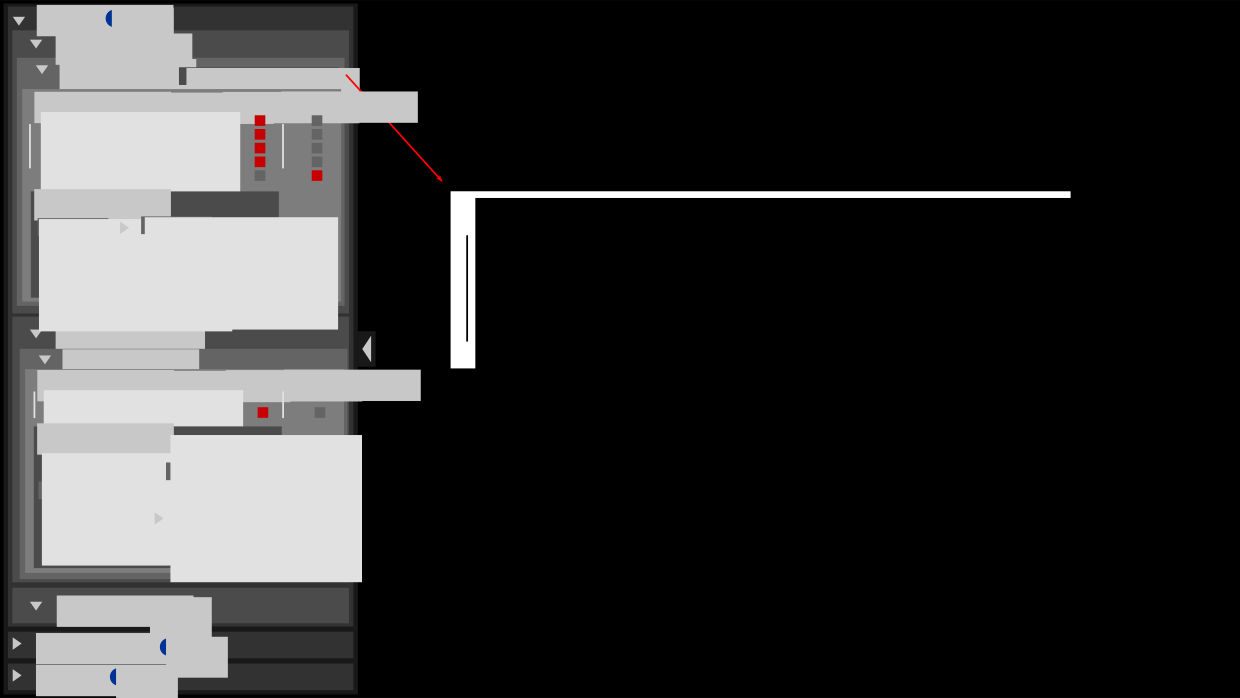
\includegraphics[scale=0.5]{sketch_2017-01-02_1}
\centering
\caption{This figure illustrates the \textbf{Query Interface} with lists of entities and properties for use in the query. It also shows an example of a table of entities along with custom properties, such as additional biological properties or experimental attributes, that the user can load from file.}
\label{fig:2017-01-02_1}
\end{figure}

% Figure 2
\begin{figure}[htbp]
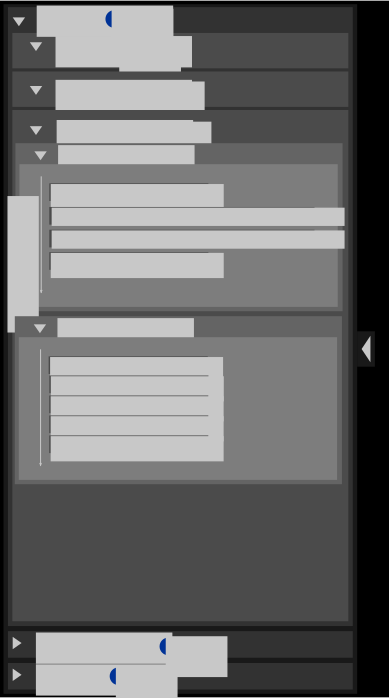
\includegraphics[scale=1]{sketch_2017-01-02_2}
\centering
\caption{This figure illustrates the \textbf{Query Interface} with sections to control the execution sequence of the query and to display results from the query.}
\label{fig:2017-01-02_2}
\end{figure}

% Figure 3
\begin{figure}[htbp]
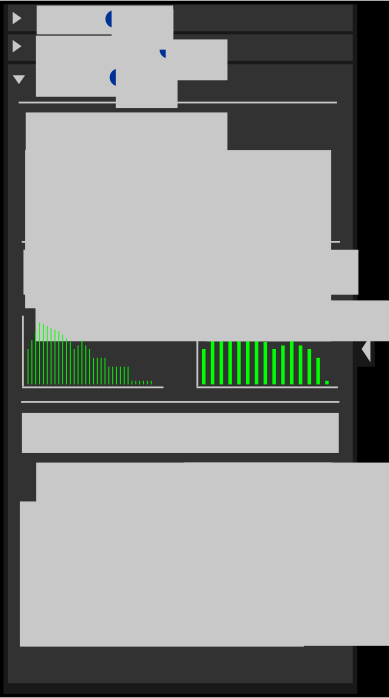
\includegraphics[scale=1]{sketch_2017-01-02_3}
\centering
\caption{This figure illustrates the \textbf{Detail Interface} with charts depicting the distribution of metabolite degrees and betweenness centralities and the distribution of metabolites between cellular compartments.}
\label{fig:2017-01-02_3}
\end{figure}

% Figure 4
\begin{figure}[htbp]
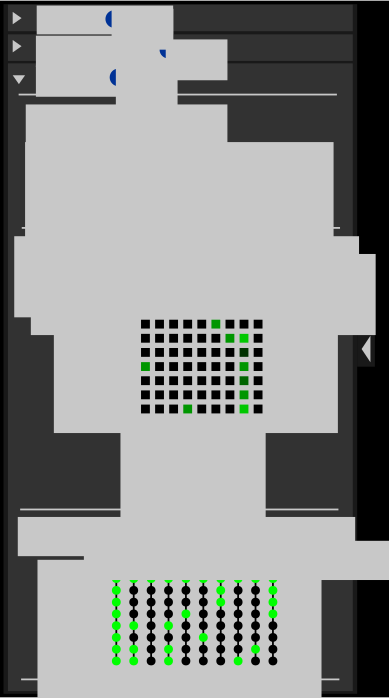
\includegraphics[scale=1]{sketch_2017-01-02_4}
\centering
\caption{This figure illustrates the \textbf{Detail Interface} with charts depicting the count of transport events between cellular compartments and the distribution of shared metabolites between combinations of multiple compartments.}
\label{fig:2017-01-02_4}
\end{figure}

% Figure 5
\begin{figure}[htbp]
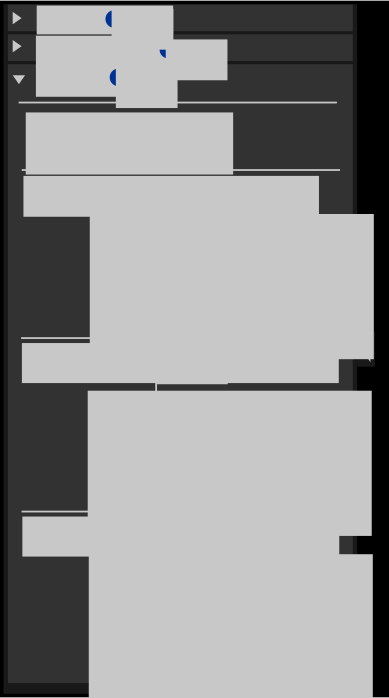
\includegraphics[scale=1]{sketch_2017-01-02_5}
\centering
\caption{This figure illustrates the \textbf{Detail Interface} with information in detail for a single metabolite.}
\label{fig:2017-01-02_5}
\end{figure}

% Figure 6
\begin{figure}[htbp]
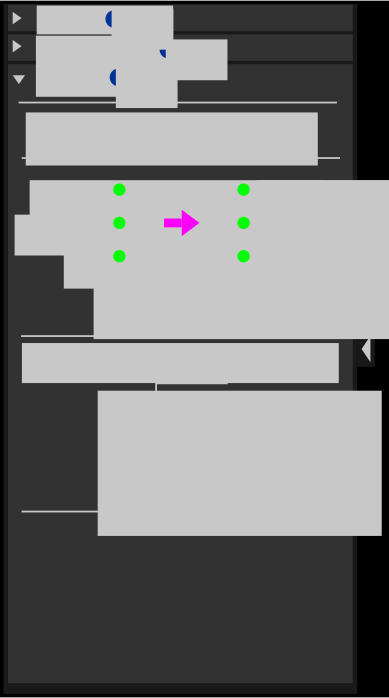
\includegraphics[scale=1]{sketch_2017-01-02_6}
\centering
\caption{This figure illustrates the \textbf{Detail Interface} with information in detail for a single reaction.}
\label{fig:2017-01-02_6}
\end{figure}

% Figure 7
\begin{figure}[htbp]
\includegraphics[scale=0.5]{sketch_2017-01-02_7}
\centering
\caption{This figure illustrates the \textbf{Navigation Interface} and the \textbf{Exploration Interface} without representation of properties by either position or color.}
\label{fig:2017-01-02_7}
\end{figure}

% Figure 8
\begin{figure}[htbp]
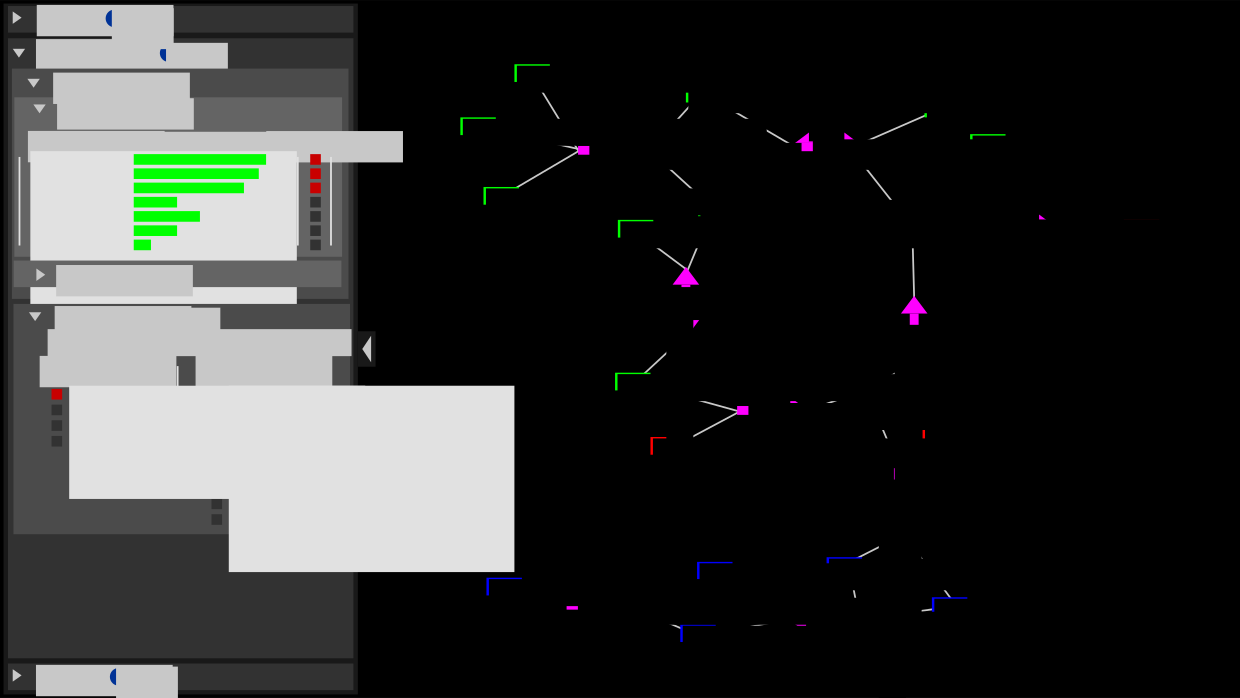
\includegraphics[scale=0.5]{sketch_2017-01-02_8}
\centering
\caption{This figure illustrates the \textbf{Navigation Interface} and the \textbf{Exploration Interface} with representation of pathway in color.}
\label{fig:2017-01-02_8}
\end{figure}

% Figure 9
\begin{figure}[htbp]
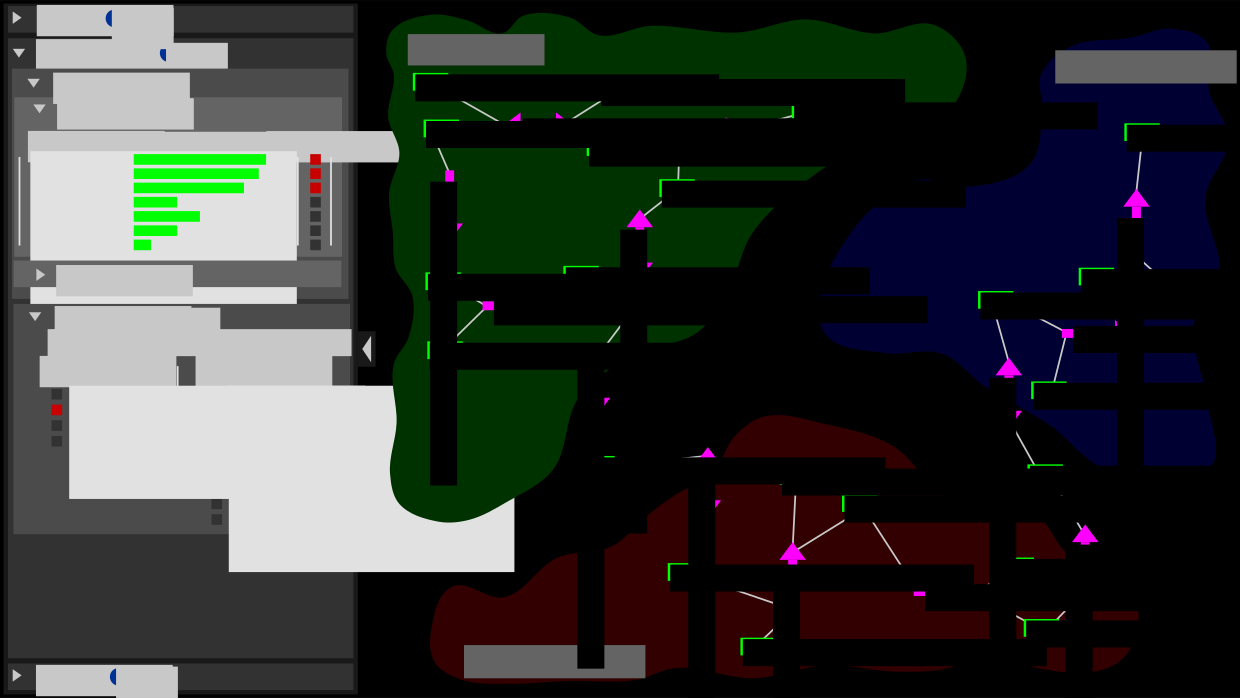
\includegraphics[scale=0.5]{sketch_2017-01-02_9}
\centering
\caption{This figure illustrates the the \textbf{Navigation Interface} and the \textbf{Exploration Interface} with representation of cellular compartment by position.}
\label{fig:2017-01-02_9}
\end{figure}

% Figure 10
\begin{figure}[htbp]
\includegraphics[scale=0.5]{sketch_2017-01-02_10}
\centering
\caption{This figure illustrates the \textbf{Navigation Interface} and the \textbf{Exploration Interface} with representation of cellular compartment by position and fold change by color.}
\label{fig:2017-01-02_10}
\end{figure}


\end{document}

%%%%%%%%%%%%%%%%%%%%%%%%%%%%%%%%%%%%%%%%%%%%%%%%%%